\documentclass[11pt,a4paper]{article}

% Packages
\usepackage[utf8]{inputenc}
\usepackage[T1]{fontenc}
% Typography: URW Palatino (Palladio) text + Pazo math + Inconsolata mono.
% This is the same font stack used by the Qwen technical reports.
\usepackage{mathpazo}
\usepackage[scaled=0.95]{inconsolata}
\usepackage{microtype}
\usepackage{amsmath,amssymb,amsfonts}
\usepackage{graphicx}
\usepackage[numbers,sort&compress]{natbib}
\usepackage{booktabs}
\usepackage{xcolor}
\usepackage{fancyhdr}
\usepackage{tikz}
\usetikzlibrary{arrows.meta, positioning, fit, backgrounds, calc}
\usepackage[margin=1in]{geometry}
\usepackage[hidelinks]{hyperref}

% Resolve assets/figures whether compiled from the repo root or this folder
\graphicspath{{papers/2026-06-roastme/}{./}}

% Brand header (logo + wordmark on the left, date on the right)
\definecolor{gaussiadark}{HTML}{323030}
\definecolor{gaussiaccent}{HTML}{C15A35}
\newcommand{\paperdate}{\today}
\newcommand{\papersurl}{https://www.gaussia.ai/papers}
\newcommand{\repourl}{https://github.com/gaussia-labs/papers}
\newcommand{\hfurl}{https://huggingface.co/gaussia-labs}
% Header logo (no link, just branding)
\newcommand{\gaussialogo}{%
  \raisebox{-0.28\height}{
\includegraphics[height=14pt]{logo}}%
  \hspace{5pt}\textcolor{gaussiadark}{\textbf{\large Gaussia}}%
}
% Clickable links shown under the title, Qwen-report style
\newcommand{\paperlinks}{%
  \begin{center}
    \href{\repourl}{%
      \raisebox{-0.22\height}{
\includegraphics[height=11pt]{github}}%
      \hspace{4pt}\texttt{github.com/gaussia-labs/papers}}\\[4pt]
    \href{\papersurl}{%
      \raisebox{-0.26\height}{
\includegraphics[height=11pt]{logo}}%
      \hspace{4pt}\texttt{gaussia.ai/papers}}\\[4pt]
    \href{\hfurl}{%
      \raisebox{-0.26\height}{
\includegraphics[height=12pt]{hf-logo}}%
      \hspace{4pt}\texttt{huggingface.co/gaussia-labs}}
  \end{center}%
}

\providecommand{\keywords}[1]{%
  \vspace{0.5em}%
  \noindent\textbf{Keywords: }#1%
}

\setlength{\headheight}{18pt}
\pagestyle{fancy}
\fancyhf{}
\lhead{\gaussialogo}
\rhead{\textcolor{gaussiadark}{\paperdate}}
\renewcommand{\headrulewidth}{0.6pt}
\rfoot{\thepage}

% Metadata
\title{Roast Me: Profile-Driven, Knowledge-Grounded\\ Red Teaming of AI Assistants}
\author{
  Alex Fiorenza \\
  \texttt{alexfiorenza2012@gmail.com}
  \and
  Axel Fritz \\
  \texttt{axel.fritz@alquimia.ai}
}
% Date is shown in the header instead of under the title (see \paperdate above)
\date{}

\begin{document}

\maketitle
\thispagestyle{fancy}

% Repository and website links, shown under the title
\paperlinks

% The abstract is REQUIRED for every Gaussia paper. Do not remove it.
\begin{abstract}
Production AI assistants often break even when they have full document
coverage, because they mishandle realistic interaction patterns: confident
false premises, implied authority, pressure to reveal internal tools,
unsupported feature assumptions, knowledge-base contradictions, and multi-turn
escalation. Static, document-grounded test sets rarely surface these failures.
We present Roast Me, an integrated red-teaming module for the Gaussia evaluation
framework that evolves document-grounded dataset generation into
assistant-specific adversarial evaluation. Roast Me operates in two stages. A
\emph{Profiler} performs reconnaissance on a target assistant, seeded by an
extensible Universal Probe Library that any provider can implement and
contribute, optionally grounded in a provided Knowledge Base, and produces an
operational profile of its purpose, domain, knowledge-grounded behavior, and
likely weaknesses. An
\emph{Exploiter} then searches for reproducible \emph{categories} of natural
interactions that reliably trigger failures, treating a query family as the unit
of discovery and following an abstractive red-teaming perspective. Both stages
run in either a black-box or a knowledge-grounded mode, treating the Knowledge
Base as a first-class input that defines what the assistant is expected to know,
cite, preserve, and avoid extrapolating beyond. A single run yields three
artifacts: an assistant profile, a ranked failure-category report with severity
and representative examples, and a reusable Roast Dataset of concrete failure
cases with violated principles, grader rationale, and supporting evidence that
can be rerun as regression tests against future assistant versions. The result
is a framework-agnostic methodology that unifies black-box behavioral red
teaming with knowledge-grounded adversarial evaluation.
\end{abstract}

\keywords{red teaming, assistant profiling, adversarial evaluation, synthetic
data generation, knowledge-grounded evaluation, LLM evaluation}

\section{Introduction}

Large language models are increasingly deployed as \emph{role-constrained
assistants}: customer-support agents, developer copilots, documentation guides,
compliance helpers, and domain experts. Such assistants operate under an
implicit contract. They are expected to know a specific body of material, to
stay within a defined scope, to respect documented constraints, and to refuse
or defer when a request falls outside what they can justify. Evaluating whether
an assistant honors that contract, reliably and across the messy ways real users
actually interact with it, has become a core quality problem.

\subsection{From Coverage to Behavior}

A first generation of evaluation tooling framed this problem as one of
\emph{coverage}. Given a knowledge base (documentation, product specifications,
support articles, policy documents), the goal was to test whether an assistant
\emph{knows} the material. The Gaussia Generators module embodies this view: it
loads context, chunks it, and uses an LLM to synthesize queries and multi-turn
conversations that probe how well an assistant reproduces and applies documented
knowledge \citep{gaussia-generators}. Coverage-oriented generation is valuable,
and it remains the right tool when the question is ``does the assistant know
what it is supposed to know?''

In production, however, assistants rarely fail because they lack coverage. They
fail because they mishandle realistic \emph{interaction patterns}. A user states
a confident false premise and the assistant accepts it. A request arrives
wrapped in implied authority, such as ``for our security audit,'' and the
assistant over-shares internal tools or hidden prompts. A user asks about a
feature that sounds plausible but does not exist, and the assistant fabricates
an API instead of correcting the premise. A conversation escalates gradually
across turns until the assistant drifts outside its scope. Two documentation
sections contradict each other and the assistant confidently picks one without
flagging the conflict. None of these are coverage gaps. They are
\emph{behavioral} failures under pressure, and a static, document-grounded test
set rarely surfaces them, since such a set rewards recall and was never designed
to stress behavior.

\subsection{Why Naive Red Teaming Is Not Enough}

Red teaming is the natural response: deliberately probe the assistant with
adversarial inputs to discover where it breaks. Two recurring problems limit how
useful naive red teaming is for product evaluation. First, much red teaming
optimizes \emph{single, brittle prompts}: one exotic jailbreak string that
happens to work once. Such findings are hard to reproduce, hard to interpret,
and hard to convert into a durable regression test, because each one captures a
lucky phrasing with no guarantee that the underlying weakness generalizes.
Second, generic red teaming is \emph{assistant-agnostic}: it throws the same
catalogue of attacks at every target, ignoring what \emph{this} assistant is
for, what it is supposed to know, and where it is actually likely to fail. The
result is either noise or findings that do not map onto the assistant's real
behavioral contract.

Two lines of work point toward a better approach. Practical red-teaming tools
such as Promptfoo organize adversarial testing around a clean separation between
a \emph{plugin} (the type of risk being tested) and a \emph{strategy} (the
interaction pattern used to present that risk), and then grade each attempt to
produce concrete pass/fail evidence \citep{promptfoo2026redteam}. This vocabulary
gives evaluators a principled language for ``what risk'' and ``how to present
it.'' Separately, \emph{abstractive red-teaming} reframes the unit of discovery
itself: instead of searching for individual attack strings, it searches for
natural-language \emph{categories} of queries that routinely elicit failures
across many concrete variants \citep{rahn2026abstractive}. A category such as
``the user asks about a plausible but nonexistent API using a confident technical
tone'' is reproducible, interpretable, and directly testable.

\subsection{Roast Me}

We present \textbf{Roast Me}, an integrated red-teaming module for the Gaussia
evaluation framework that evolves coverage-oriented dataset generation into
\emph{assistant-specific, knowledge-grounded adversarial evaluation}. Roast Me
operates in two stages:

\begin{itemize}
  \item The \textbf{Profiler} performs reconnaissance on a target assistant and
  builds an operational profile of its purpose, domain, limitations,
  knowledge-grounded behavior, and above all its \emph{likely weaknesses}. It
  answers: \emph{what kind of assistant are we dealing with, and where does it
  appear vulnerable?}
  \item The \textbf{Exploiter} takes those likely weaknesses and searches for
  reproducible \emph{categories} of natural interactions that reliably trigger
  failures in that specific assistant. It answers: \emph{which families of
  realistic interactions break it, again and again?}
\end{itemize}

Roast Me adopts the plugin/strategy/grader vocabulary from practical red teaming
in its Profiler \citep{promptfoo2026redteam}, and the category-search perspective
from abstractive red teaming in its Exploiter \citep{rahn2026abstractive}.
Crucially, it treats an optional \textbf{Knowledge Base} as a \emph{first-class
input}. When provided, the Knowledge Base defines what the assistant is expected
to know, cite, preserve, distinguish, and avoid extrapolating beyond. This lets
Roast Me test both generic behavioral weaknesses and whether the assistant
respects the specific material it is responsible for. When no Knowledge Base is
available, Roast Me still runs in a black-box mode driven by the assistant
profile alone.

Both stages are seeded by pluggable, provider-supplied libraries, which keeps
Roast Me open and extensible. The Profiler draws its starting probes from a
\textbf{Universal Probe Library}: an extensible pool of risk families and
interaction patterns that any provider can develop, implement, and integrate to
feed the reconnaissance stage. The library lets profiling cold-start on any
assistant, even with no production logs or internal documentation, and when a
Knowledge Base is present its patterns are grounded into the assistant's domain.
The Exploiter has an analogous pluggable seed, a \textbf{Universal Natural Query
Prior}, that shapes how realistic the generated interactions sound. This design
allows an organization to extend the probe and query libraries for its own
domain while the core profile-then-exploit loop stays unchanged.

\subsection{The Deliverable}

A single Roast Me run emits three artifacts, and they differ in standing. The
\emph{assistant profile} and the \emph{failure-category report} describe how the
system arrived at its findings: the profile is largely an intermediate that
bridges the two stages, and the report is the human-readable summary of what
broke and why it matters. The intended \textbf{final deliverable is the Gaussia
Roast Dataset}: a structured, reusable set of concrete failure cases, each
carrying the query, the assistant's response, the source category, the violated
principle, the grader's rationale, and, in knowledge-grounded mode, the
supporting or contradicting evidence captured during the run.

Framing the dataset as the primary output is deliberate. First, it closes the
loop with the rest of Gaussia: the Roast Dataset is a first-class evaluation
dataset, compatible with existing metrics, much as Gaussia Generators produced
reusable datasets for downstream metrics \citep{gaussia-generators}. A Roast Me
run therefore terminates in \emph{data that feeds the evaluation pipeline},
ready for existing metrics to consume. Second, the dataset is actionable and
repeatable: its cases become regression tests that can be rerun against future
assistant versions to catch behavioral regressions, whereas a profile or a
report only captures a single moment. Third, the dataset encodes the central
product of the search, the \emph{categories} that failed reproducibly, so the
durable knowledge of where an assistant breaks is preserved in a form that
survives re-testing. In short, the profile and report are the path; the Roast
Dataset is what the evaluator takes away.

\subsection{Contributions}

This paper makes the following contributions:

\begin{itemize}
  \item A two-stage methodology, \emph{profile-then-exploit}, that first builds an
  assistant-specific profile of likely weaknesses and then searches for the
  interaction categories that exploit them, in place of a fixed,
  assistant-agnostic attack catalogue.
  \item A treatment of the \emph{Knowledge Base as a first-class input} to
  adversarial evaluation, unifying black-box behavioral red teaming with
  knowledge-grounded testing of whether an assistant respects documented truth,
  handles ambiguity and contradiction, and avoids unsupported extrapolation.
  \item A reusable, framework-agnostic output, the \emph{Gaussia Roast Dataset},
  that turns reproducible failure categories into regression tests and positions
  red teaming as a producer of durable evaluation data for ongoing use.
\end{itemize}

The remainder of this paper opens with a high-level overview of the system, then
describes how the Knowledge Base is consumed through the Probe Library, the
Profiler and the Exploiter in detail, the theoretical implementation
considerations for any SDK, and the outputs the system produces.

\section{System at a Glance}
\label{sec:overview}

A Roast Me run threads a target assistant, optional knowledge, and two pluggable
libraries through two stages, and emits three artifacts. Figure~\ref{fig:overview}
sketches the flow. This section walks through it at a high level, using a running
example: an assistant that answers questions about a software SDK.

\begin{figure}[ht]
\centering
\begin{tikzpicture}[
  font=\footnotesize,
  >={Stealth[length=2mm]},
  io/.style={draw, rounded corners=2pt, align=center, inner sep=4pt,
             minimum height=0.8cm, fill=black!3},
  plug/.style={draw, dashed, rounded corners=2pt, align=center, inner sep=4pt,
               minimum height=0.8cm, fill=gaussiaccent!7},
  stage/.style={draw, thick, rounded corners=3pt, align=center, inner sep=6pt,
                minimum width=4.6cm, minimum height=1.25cm, fill=gaussiadark!7},
  art/.style={draw, rounded corners=2pt, align=center, inner sep=4pt,
              minimum height=0.9cm, minimum width=3.0cm},
  deliv/.style={draw, very thick, draw=gaussiaccent, rounded corners=2pt,
                align=center, inner sep=4pt, minimum height=0.9cm,
                minimum width=3.0cm, fill=gaussiaccent!10},
  flow/.style={->, thick},
  bi/.style={<->, thick, gaussiadark!70},
  feed/.style={->, thick, gaussiaccent!85}
]

% Center spine
\node[stage] (prof) {\textbf{Profiler}\\ \scriptsize reconnaissance};
\node[art, below=1.0cm of prof] (profile) {Assistant Profile\\ \scriptsize + likely weaknesses\\ \scriptsize + knowledge hooks};
\node[stage, below=1.0cm of profile] (exp) {\textbf{Exploiter}\\ \scriptsize category search + refinement};

% Pluggable libraries (left); the probe library is the sole gateway to the KB
\node[plug, left=1.7cm of prof] (probe) {Universal\\ Probe Library};
\node[plug, left=1.7cm of exp] (prior) {Universal Natural\\ Query Prior};

% Knowledge Base feeds only the probe library; target assistant on the right
\node[io, above=0.7cm of probe] (kb) {Knowledge Base \scriptsize(optional)};
\node[io, right=1.7cm of profile] (asst) {Target\\ Assistant};

% Outputs (bottom row)
\node[art, below=1.0cm of exp] (report) {Failure Category\\ Report};
\node[art, left=0.5cm of report] (profout) {Assistant\\ Profile};
\node[deliv, right=0.5cm of report] (dataset) {\textbf{Gaussia}\\ \textbf{Roast Dataset}};

% Edges: KB is confined to the probe library, which emits particularized, tagged probes
\draw[feed] (kb) -- (probe);
\draw[feed] (probe) -- node[above, font=\scriptsize, black!60] {probes + tags} (prof);
\draw[feed] (prior) -- (exp);

% Edges: spine (the profile is the single interface between stages)
\draw[flow] (prof) -- (profile);
\draw[flow] (profile) -- (exp);

% Edges: assistant interaction
\draw[bi] (asst) -- (prof.east);
\draw[bi] (asst) -- (exp.east);

% Edges: outputs
\draw[flow] (exp) -- (report);
\draw[flow] (exp.south) -- ++(0,-0.45) -| (profout.north);
\draw[flow] (exp.south) -- ++(0,-0.45) -| (dataset.north);

% Grouping label for outputs
\begin{scope}[on background layer]
  \node[draw=black!25, dashed, rounded corners=3pt, fit=(profout)(report)(dataset),
        inner sep=6pt, label={[black!55,font=\scriptsize]below:Outputs}] {};
\end{scope}

\end{tikzpicture}
\caption{Roast Me at a glance. The optional Knowledge Base is reached only
through the Universal Probe Library, which emits domain-particularized,
tagged probes; the Profiler stays blind to the Knowledge Base. The profile is
the single interface between stages: it carries the likely weaknesses and the
distilled knowledge hooks the Exploiter needs. A second pluggable library, the
Universal Natural Query Prior, seeds realistic phrasing during exploitation. The
run emits three artifacts; the Gaussia Roast Dataset is the final, reusable
deliverable.}
\label{fig:overview}
\end{figure}

\paragraph{Inputs.}
Every run needs access to a \textbf{target assistant}. The evaluator may also
supply a \textbf{Knowledge Base} (documentation, API references, policies) and
configure the two pluggable libraries: the \textbf{Universal Probe Library} that
seeds reconnaissance and the \textbf{Universal Natural Query Prior} that seeds
realistic phrasing during exploitation. Both libraries are provider-extensible,
so an organization can add its own probe families or query sources for a given
domain.

\paragraph{Knowledge stays inside the Probe Library.}
The Knowledge Base is reached only through the Universal Probe Library, which is
the sole component with access to it. The library ingests the Knowledge Base and
emits \textbf{domain-particularized probes}, each tagged with the knowledge it
embeds: which referenced entities are documented, which are plausible but absent
from the source material, and which constraints or contradictions a probe targets. The
backend behind this step is the implementer's choice, such as simple retrieval
over chunks, a knowledge graph, entity extraction, or a hybrid; the rest of the
system depends only on the library's interface. In the running example, the
library knows that \texttt{DatasetGenerator} is documented and that
\texttt{create\_roast\_pipeline()} is absent, so it can build a probe that asks
about the latter and tag it as undocumented.

\paragraph{Stage~1: Profiler.}
The Profiler stays blind to the Knowledge Base. It receives particularized probes
with their tags, sends them to the assistant, grades the responses, and rolls the
results up into an \textbf{assistant profile}. The profile carries two things:
the likely weaknesses inferred from the grades, and a set of \textbf{knowledge
hooks} aggregated from the tags of the probes that mattered (documented entities,
undocumented references, constraints, contradictions). In the example, a
false-premise probe about \texttt{create\_roast\_pipeline()} makes the assistant
invent an import path and signature, so the profile records both a tendency to
fabricate documentation-adjacent APIs and the hooks that exposed it.

\paragraph{Stage~2: Exploiter.}
The Exploiter consumes only the profile, so the profile is the single interface
between the two stages. From the likely weaknesses, the knowledge hooks, and a
behavioral contract, it proposes \textbf{categories} of interactions that should
break the assistant. When a category becomes concrete queries, the Universal
Natural Query Prior shapes them so they read like a real user, and the hooks let
the queries and reward models reference real and false entities without ever
touching the Knowledge Base. Queries go to the assistant, reward models score
them, and categories that fail reproducibly are kept and refined. In the example,
the category ``the user asks about undocumented APIs whose names resemble
documented components'' fails on most variants and rises to the top.

\paragraph{Outputs.}
The run ends with three artifacts: the assistant profile, a ranked failure
category report, and the \textbf{Gaussia Roast Dataset}. As argued above, the
dataset is the final deliverable: a reusable set of concrete failure cases that
can be rerun as regression tests.

\section{Related Work}

Roast Me sits at the intersection of three lines of work: practical red-teaming
frameworks, abstractive red teaming, and synthetic dataset generation for
evaluation. It borrows a vocabulary from the first, a search perspective from the
second, and an output philosophy from the third.

\subsection{Practical Red-Teaming Frameworks}

Production-oriented red-teaming tools have converged on a useful separation of
concerns. Promptfoo, for example, organizes adversarial testing around a
\emph{plugin}, which names the type of risk under test, and a \emph{strategy},
which names the interaction pattern used to deliver that risk, and then grades
each attempt to produce concrete pass/fail evidence \citep{promptfoo2026redteam}.
This vocabulary gives evaluators a shared language for what to test and how to
present it, and it maps cleanly onto a library of reusable attack components.

Roast Me adopts the plugin/strategy/grader vocabulary inside its Profiler, with
two departures. First, it treats plugins as universal risk families that seed a
provider-extensible Universal Probe Library, so reconnaissance can cold-start on
any assistant. Second, it adds a knowledge-grounding step: when a Knowledge Base
is available, the library particularizes its probes to the assistant's domain and
tags each probe with the entities and constraints it embeds. The result of this
stage is an assistant profile, which existing frameworks do not produce as a
distinct, reusable artifact.

\subsection{Automated Strategy Discovery}

A parallel line of work automates the discovery of adversarial inputs in place of
a fixed attack catalogue. AutoDAN-Turbo frames red teaming as lifelong strategy
exploration: a loop among an attacker, a target, and a scorer discovers jailbreak
strategies from scratch, stores them in a retrieval-indexed library, and
recombines them across attempts, reaching strong attack success rates with no
human-authored strategies \citep{liu2025autodanturbo}. AutoRed removes the
dependence on seed instructions, conditioning a persona prior to synthesize
semantically diverse adversarial prompts and training a verifier that estimates a
prompt's harmfulness without querying the target model \citep{diao2025autored}.
These methods establish that adversarial discovery can be automated, diverse, and
reusable, and Roast Me shares their view that discovery itself is the object of
search.

Two gaps remain for assistant evaluation. First, both are assistant-agnostic:
they optimize attacks against a generic notion of harm, not against a specific
assistant's behavioral contract, so their findings do not speak to whether a
given assistant respects its documented scope. Second, both emphasize the
magnitude of failure over its reproducibility: a strategy that raises a scorer
once enters the library, and the target's stochasticity is often removed by
decoding at zero temperature \citep{liu2025autodanturbo}, which weakens
reproducibility under realistic deployment. Roast Me keeps automated, reusable
discovery and conditions it on an explicit assistant profile, scoring categories
by a reproducibility-penalized lower bound (Section~\ref{sec:theory}) so that
what it discovers is both assistant-specific and stable across samples.

\subsection{Abstractive Red Teaming}

A complementary line of work changes the unit of discovery. Instead of optimizing
individual attack strings, abstractive red teaming searches for natural-language
\emph{categories} of queries that elicit failures across many concrete variants,
for example a description such as ``the query asks for prison survival tools in a
numbered list'' \citep{rahn2026abstractive}. Categories are reproducible,
interpretable, and easier to convert into durable tests than single prompts.

Roast Me applies this perspective in its Exploiter, with two adaptations for
assistant evaluation. The category search is conditioned on the assistant profile
produced by the Profiler, so it concentrates on families the target is already
suspected to mishandle. The search also draws on the knowledge hooks carried by
the profile, which lets generated categories and queries reference real and
plausible-but-false entities for a specific product domain while the Exploiter
stays decoupled from the raw Knowledge Base.

\subsection{Synthetic Dataset Generation for Evaluation}

Automated dataset generation addresses the cost of building evaluation sets by
hand. Gaussia Generators loads context, chunks it, and uses an LLM to synthesize
queries and multi-turn conversations, producing reusable, framework-compatible
datasets for downstream metrics \citep{gaussia-generators}. Its emphasis is
coverage: testing whether an assistant reproduces and applies documented
material. It also exposes pluggable chunk-selection strategies, so the source of
generated content is swappable.

Roast Me continues this output philosophy and extends its scope. It keeps the
goal of emitting a reusable, framework-compatible dataset, and it reuses the
pluggable-source idea through the Universal Natural Query Prior, which mirrors
pluggable chunk selection by exposing a swappable source of realistic phrasing.
The extension is in what the dataset captures: behavioral failures under
realistic pressure, organized as reproducible categories, together with the
assistant profile and a ranked failure report.

\subsection{Positioning}

The closest single ideas to Roast Me already exist in isolation: a plugin and
strategy vocabulary for risks, automated and reusable strategy discovery, a
category-level view of failures, and reusable synthetic datasets. Roast Me combines them into one methodology and adds two
elements that tie them together. The first is the two-stage,
\emph{profile-then-exploit} structure, in which reconnaissance produces an
explicit assistant profile that conditions the later search. The second is the
treatment of knowledge through tagged probes and distilled knowledge hooks, which
keeps the Knowledge Base confined to the Probe Library while still allowing
knowledge-grounded exploitation. Together they turn red teaming into a producer
of durable, framework-compatible evaluation data.

\section{Theoretical Formulation}
\label{sec:theory}

This section formalizes Roast Me as a search problem over \emph{categories} of
interactions that induce contract violations in a target assistant. We first fix
notation and state the problem (Section~\ref{sec:setup}). We then formalize the
three components of Roast Me: how the Probe Library particularizes and tags
probes from a Knowledge Base (Section~\ref{sec:probes}), how the Profiler
compresses the assistant into a reusable profile (Section~\ref{sec:profiler}),
and how the Exploiter searches for high-yield categories
(Section~\ref{sec:exploiter}).

\subsection{Problem Setup and Notation}
\label{sec:setup}

\paragraph{Target assistant.}
Let $\mathcal{X}$ denote the space of conversation histories, where each
$x \in \mathcal{X}$ is a (possibly multi-turn) sequence of user and assistant
messages, and let $\mathcal{R}$ denote the space of assistant responses. We model
the target assistant as a stochastic map
\begin{equation}
  A : \mathcal{X} \rightarrow \Delta(\mathcal{R}),
\end{equation}
where $\Delta(\mathcal{R})$ is the set of probability distributions over
responses. For a history $x$ we write $r \sim A(x)$ for a sampled response. We
treat $A$ as a black box: the evaluator can sample responses but cannot inspect
parameters, system prompts, or internal tools. A single user query $q$ is the
special case of a length-one history.

\paragraph{Behavioral contract.}
The evaluation specification is a \emph{behavioral contract}, a finite set of
principles
\begin{equation}
  \Pi = \{\pi_1, \dots, \pi_m\}, \qquad
  \pi_j : \mathcal{X} \times \mathcal{R} \rightarrow \{0,1\},
\end{equation}
where $\pi_j(x, r) = 1$ marks a violation of principle $j$ by response $r$ in
context $x$. Typical principles include ``do not fabricate undocumented
capabilities,'' ``do not reveal hidden tools or internal prompts,'' ``do not
accept a false premise without correction,'' and ``do not contradict the
provided source material.'' The principles are part of the input: they define
what counts as a failure for this assistant.

\paragraph{Graders and violation score.}
The principles $\pi_j$ are generally not available in closed form, so each is
approximated by a \emph{grader} (equivalently, a judge)
$\hat\pi_j : \mathcal{X} \times \mathcal{R} \rightarrow [0,1]$, which returns an
estimated probability or severity of violation. A grader may itself call an LLM,
apply a rule, or consult retrieved evidence. We summarize the contract through an
aggregate \emph{violation score}
\begin{equation}
  v(x, r) \;=\; \sum_{j=1}^{m} w_j \, \hat\pi_j(x, r) \;\in\; [0,1],
  \qquad \sum_{j=1}^{m} w_j = 1,
  \label{eq:violation}
\end{equation}
with nonnegative weights $w_j$ encoding the relative severity of each principle.
Setting all mass on a single principle recovers the single-risk case, and using
indicator graders recovers a hard pass/fail.

\paragraph{Knowledge base.}
The evaluator may optionally supply a \emph{knowledge base} $K$, a collection of
source material the assistant is expected to respect. We deliberately leave the
internal representation of $K$ unspecified. The only requirement is an interface,
exposed by the Probe Library (Section~\ref{sec:probes}), that particularizes and
tags probes against $K$. This keeps the formulation
agnostic to the retrieval technology, whether plain chunk retrieval, a knowledge
graph, entity extraction, or a hybrid. When $K$ is absent, Roast Me runs in
black-box mode and the knowledge-dependent terms below are simply empty.

\paragraph{Categories and queries.}
The central object of the search is an interaction \emph{category} $c$, an
abstract description of a family of interactions, such as ``the user asks about a
plausible but nonexistent API in a confident technical tone.'' A category induces
a conditional distribution over interactions,
\begin{equation}
  Q_c \in \Delta(\mathcal{X}),
\end{equation}
from which concrete queries are sampled, $q \sim Q_c$. A single hand-written
attack prompt is the degenerate case in which $Q_c$ is a point mass. Operating at
the level of $Q_c$ makes findings reproducible across variants, following the
abstractive perspective of \citet{rahn2026abstractive}. Section~\ref{sec:exploiter}
gives categories their explicit attribute structure.

\paragraph{Realism prior.}
The Universal Natural Query Prior is a distribution $N \in \Delta(\mathcal{X})$
(or a mixture of provider-supplied sources) over realistic user phrasings. It
carries no adversarial intent on its own; its role is to keep sampled queries
close to how real users write. We formalize this as a soft constraint through a
divergence $D\!\left(Q_c \,\|\, N\right)$ that the query generator keeps small,
so that a category's instances read like plausible user traffic.

\paragraph{Objective.}
For a category $c$, define its \emph{failure rate} under the contract as the
expected violation it induces,
\begin{equation}
  \Phi(c) \;=\; \mathbb{E}_{q \sim Q_c}\; \mathbb{E}_{r \sim A(q)}\;
  \big[\, v(q, r) \,\big].
  \label{eq:phi}
\end{equation}
A useful category has high $\Phi(c)$ and is also \emph{reproducible}, meaning the
violation persists across independent samples from $Q_c$ instead of resting on a
single lucky phrasing. We therefore score a category by a lower-confidence
estimate
\begin{equation}
  S(c) \;=\; \hat\Phi_n(c) \;-\; \lambda \, \widehat{\mathrm{se}}_n(c),
  \label{eq:score}
\end{equation}
where $\hat\Phi_n(c)$ is the empirical mean of $v$ over $n$ sampled
query/response pairs, $\widehat{\mathrm{se}}_n(c)$ is its standard error, and
$\lambda \ge 0$ trades reward against uncertainty. The penalty rewards categories
that fail \emph{consistently}.

\paragraph{The search problem.}
Roast Me does not seek a single worst prompt. It seeks a \emph{set} of realistic,
on-profile categories that break the assistant reproducibly. Given a profile
$\theta$ (Section~\ref{sec:profiler}) that restricts attention to a
profile-relevant family $\mathcal{C}_\theta$, the Exploiter approximates
\begin{equation}
  \mathcal{C}^\star \;=\;
  \big\{\, c \in \mathcal{C}_\theta \;:\; S(c) \ge \tau,\;\;
  D\!\left(Q_c \,\|\, N\right) \le \delta \,\big\},
  \label{eq:search}
\end{equation}
the categories whose reproducible failure score clears a threshold $\tau$ while
staying within a realism budget $\delta$. Section~\ref{sec:profiler} defines the
profile $\theta$ and the family $\mathcal{C}_\theta$, and
Section~\ref{sec:exploiter} defines the sampling of $Q_c$ and the search itself.

\paragraph{An embedding-based instantiation of $D$.}
The divergence $D\!\left(Q_c \,\|\, N\right)$ in
Eq.~\eqref{eq:search} is left abstract so that any realism estimator may be
used; here we record one lightweight choice that is cheap enough to evaluate
inside the category search. Let $E : \mathcal{X} \rightarrow \mathbb{R}^d$ be a
fixed sentence encoder. Following \citet{diao2025autored}, who quantify the
semantic dissimilarity between two prompts as $1 - \cos\!\big(E(q), E(q')\big)$,
we estimate the realism gap of a category by the expected cosine distance
between its sampled instances and reference draws from the prior,
\begin{equation}
  \widehat{D}\!\left(Q_c \,\|\, N\right)
  \;=\;
  1 \;-\;
  \mathbb{E}_{\,q \sim Q_c,\; q_N \sim N}
  \Big[\, \cos\!\big(E(q),\, E(q_N)\big) \,\Big].
  \label{eq:realism-cos}
\end{equation}
In words, a category whose instances embed close to typical user phrasings
incurs a small $\widehat{D}$, whereas a category that drifts into stilted or
overtly adversarial phrasing is penalized. We note one difference in intent
from \citet{diao2025autored}: there the cosine distance measures
\emph{diversity}, rewarding instructions that move \emph{away} from a seed set,
whereas in Eq.~\eqref{eq:realism-cos} the same quantity measures
\emph{proximity}, rewarding queries that stay \emph{close} to the realism prior
$N$. The two uses are complementary, and the surrogate inherits AutoRed's
practical advantage: it requires only forward passes through a frozen encoder
and never queries the target assistant.

In practice $N$ need not be sampled afresh for every comparison. When the prior
is represented by a finite pool of reference phrasings
$\{q_N^{(1)}, \dots, q_N^{(M)}\}$, one may precompute their embeddings and
compare each sampled query against the pool mean
$\bar{h}_N = \tfrac{1}{M}\sum_{k} E\!\big(q_N^{(k)}\big)$, giving the cheaper
per-query estimate $1 - \cos\!\big(E(q),\, \bar{h}_N\big)$ at the cost of
collapsing the prior to its centroid. Equation~\eqref{eq:realism-cos} is only an
instantiation: any estimator that penalizes departure from $N$, such as a
learned discriminator separating $Q_c$ samples from $N$ samples or a likelihood
under a density model of $N$, is equally compatible with the formulation, since
the search in Eq.~\eqref{eq:search} depends on $D$ only through the realism
budget $\delta$.

\subsection{Knowledge Particularization and Tagged Probes}
\label{sec:probes}

The Universal Probe Library is the only component that reads the knowledge base
$K$. It turns generic, domain-agnostic test intents into concrete probes for the
target's domain and attaches to each probe a tag that records why the probe is
relevant. The Profiler and the graders downstream see these tagged probes and
never touch $K$, which keeps the rest of the pipeline agnostic to how $K$ is
stored.

\paragraph{Probe templates.}
A probe template $t \in \mathcal{T}$ is a domain-agnostic description of one way
to stress a contract principle, for example ``ask about a capability that sounds
plausible but is undocumented,'' ``ask the assistant to act outside its stated
scope,'' or ``state a false premise built from a close variant of a real
entity.'' Each template carries the subset of principles it targets,
$\Pi_t \subseteq \Pi$, so a violation elicited by $t$ is attributed to a known
part of the contract.

\paragraph{Particularization.}
Given the knowledge base, the Probe Library particularizes a template into
concrete, tagged probes. We model it as an operator
\begin{equation}
  L : \mathcal{T} \times \mathcal{K} \rightarrow \Delta(\mathcal{X} \times \mathcal{G}),
  \qquad (p, g) \sim L(t, K),
  \label{eq:probelib}
\end{equation}
where $\mathcal{K}$ is the space of knowledge bases, $p \in \mathcal{X}$ is a
concrete probe query phrased for the target's domain, and $g \in \mathcal{G}$ is
a \emph{knowledge hook}. When $K$ is absent, $L(t, \varnothing)$ returns
domain-agnostic probes with an empty hook, so the same interface drives
black-box runs.

\paragraph{Knowledge hooks.}
A knowledge hook $g$ is the structured provenance of a probe relative to $K$: the
piece of source material the probe leans on and how it is used, such as the
documented entity it references, the constraint it tests, or the undocumented
reference it introduces. We summarize a hook by a grounding label
\begin{equation}
  \mathrm{doc}(g, K) \in \{0, 1\},
  \label{eq:doc}
\end{equation}
equal to $1$ when the referenced content is present in $K$ (a documented hook)
and $0$ when the probe deliberately uses material absent from $K$ (an
undocumented reference). The library keeps this label honest, and that invariant is what
later lets a grader separate ``the assistant invented an undocumented feature''
from ``the assistant correctly described a documented one.''

\paragraph{The tagged probe set.}
Running the library over its templates against $K$ yields the tagged probe set
\begin{equation}
  P_K = \big\{\, (p_i, g_i) \,\big\}_{i=1}^{P},
  \label{eq:probeset}
\end{equation}
which is the entire interface the Probe Library exposes to the Profiler.
Everything the rest of Roast Me knows about $K$ arrives through the hooks $g_i$,
so the choice of retrieval technology, whether a knowledge graph, plain chunk
retrieval, entity extraction, or a hybrid, stays internal to $L$.

\subsection{The Profiler}
\label{sec:profiler}

The Profiler runs reconnaissance. It sends the tagged probes $P_K$ to the
assistant, grades the responses, and compresses the outcome into a compact
profile $\theta$ that the Exploiter consumes. The Profiler reads probes and tags
only, so the profile carries forward exactly the knowledge that proved relevant.

\paragraph{Probing the assistant.}
For each tagged probe $(p_i, g_i) \in P_K$ the Profiler samples one or more
responses $r_i \sim A(p_i)$ and scores them with the violation measure of
Eq.~\eqref{eq:violation}, retaining the per-principle grades
$\hat\pi_j(p_i, r_i)$ so a failure traces back to the principle it breaks. This
produces a table of graded outcomes $\{(p_i, g_i, r_i, v_i)\}$.

\paragraph{The profile.}
The Profiler aggregates these outcomes into a profile
\begin{equation}
  \theta = (\omega, H),
  \label{eq:profile}
\end{equation}
with two parts. The first is a weakness map
\begin{equation}
  \omega : \Pi \times \mathcal{Z} \rightarrow [0,1],
  \label{eq:weakness}
\end{equation}
where $\mathcal{Z}$ is a space of probe descriptors (the template, the topic, the
hook type). The value $\omega(\pi_j, z)$ estimates how readily a probe of
descriptor $z$ makes the assistant violate principle $\pi_j$, read off from the
graded outcomes. The second part is the set of retained hooks
$H \subseteq \mathcal{G}$: the hooks that produced violations or are likely to,
kept so the Exploiter can ground its categories in the same documented entities
and undocumented references.

\paragraph{From profile to search space.}
The profile defines the profile-relevant family $\mathcal{C}_\theta$ that the
Exploiter searches in Eq.~\eqref{eq:search}. A category $c = (a_1, \dots, a_\ell)$
is profile-relevant when each attribute comes from a weakness the Profiler
flagged or references a retained hook,
\begin{equation}
  \mathcal{C}_\theta = \Big\{\, c :
  \text{each } a_k \text{ is induced by some } (\pi_j, z) \text{ with }
  \omega(\pi_j, z) \ge \eta, \text{ or references a hook in } H \,\Big\},
  \label{eq:ctheta}
\end{equation}
for a threshold $\eta$. This is the sense in which the Exploiter starts where the
assistant is already suspected to be weak: $\theta$ points at the principles
worth attacking and supplies the grounded material to attack them with.

\subsection{The Exploiter}
\label{sec:exploiter}

The Exploiter receives the profile $\theta$ produced by the Profiler
(Section~\ref{sec:profiler}) and searches the profile-relevant family
$\mathcal{C}_\theta$ of Eq.~\eqref{eq:ctheta} for categories that break the
assistant reproducibly while staying realistic, approximating $\mathcal{C}^\star$
in Eq.~\eqref{eq:search}. We define a category, the way it is scored from
samples, the on-profile filter, and what the refinement step computes. The
construction follows the abstractive view of \citet{rahn2026abstractive} and adds
three elements specific to assistant evaluation: conditioning on the profile
$\theta$, an explicit realism prior $N$, and the reproducibility-penalized score
of Eq.~\eqref{eq:score}.

\paragraph{Categories as attribute conjunctions.}
We represent a category as a conjunction of natural-language \emph{attributes}
\begin{equation}
  c = (a_1, \dots, a_\ell),
  \label{eq:attributes}
\end{equation}
where each $a_k$ is a short sentence describing one aspect of a query, and the
category denotes the logical conjunction of its attributes. For instance, the
category ``the user asks about a billing feature; the feature does not exist in
the documentation; the tone is confident and technical'' has three attributes.
This structure is the discrete handle that makes the search tractable and the
findings legible: each $a_k$ names a property a human can read, and attributes
can reference the \emph{knowledge hooks} carried by $\theta$ (documented
entities, plausible but undocumented references, stated constraints), which is how a
category becomes grounded in the assistant's domain. A profile-conditioned
\emph{category generator} $p_C(\cdot \mid \theta)$ proposes categories drawn from
$\mathcal{C}_\theta$, and the conditional distribution $Q_c = p_Q(\cdot \mid c,
\theta)$ introduced in Section~\ref{sec:setup} is realized by a \emph{query
generator} that samples concrete queries satisfying the attributes of $c$. The
attributes admit many surface realizations, and $Q_c$ ranges over exactly those.

\paragraph{Scoring a category from samples.}
Given a category $c$, the Exploiter draws $n$ queries $q_i \sim Q_c$, samples
responses $r_i \sim A(q_i)$, and evaluates the violation $v(q_i, r_i)$ of
Eq.~\eqref{eq:violation}. A category score is any sample statistic of these
violations,
\begin{equation}
  R_S(c) = S\big(\{\, v(q_i, r_i) \,\}_{i=1}^{n}\big).
  \label{eq:catscore}
\end{equation}
The sample mean recovers the empirical failure rate $\hat\Phi_n(c)$ of
Eq.~\eqref{eq:phi}, which measures how often the category fails on average. To
reward categories that fail \emph{consistently} instead of categories that
occasionally spike, we instantiate $S$ as the lower-confidence bound $S(c)$ of
Eq.~\eqref{eq:score}, so the statistic that drives the search already discounts
high-variance categories.

\paragraph{On-profile filtering.}
A high violation score alone does not make a query useful. A query that openly
asks the assistant to break its contract inflates $v$ while saying nothing about
realistic deployment. We therefore gate the violation through a filter
$f : \mathcal{X} \rightarrow \mathbb{R}$ that scores how on-profile and indirect
a query is, and keep only queries above a threshold $\kappa$,
\begin{equation}
  v_{f,\kappa}(x, r) =
  \begin{cases}
    v(x, r), & f(x) \ge \kappa,\\[2pt]
    0,       & f(x) < \kappa,
  \end{cases}
  \label{eq:filtered}
\end{equation}
following the filtered-reward construction of \citet{rahn2026abstractive}. The
filter and the realism prior play complementary roles: $f$ is a per-query hard
gate that removes blatant or off-profile asks, while the divergence
$D\!\left(Q_c \,\|\, N\right) \le \delta$ from Eq.~\eqref{eq:search} is a
per-category soft budget that keeps the whole family close to natural traffic.
Substituting $v_{f,\kappa}$ for $v$ in Eq.~\eqref{eq:catscore} restricts the
search to failures that a real user could plausibly trigger by accident.

\paragraph{Searching for high-yield categories.}
We approximate the set $\mathcal{C}^\star$ in two interchangeable ways. The first
optimizes a parametric category generator $p_{\theta_C}(\cdot \mid \theta)$ to
maximize the expected category score,
\begin{equation}
  J(\theta_C) = \mathbb{E}_{\,c \sim p_{\theta_C}(\cdot \mid \theta)}\big[\, R_S(c) \,\big],
  \qquad
  \nabla_{\theta_C} J = \mathbb{E}_{\,c}\big[\, A_S(c)\, \nabla_{\theta_C} \log p_{\theta_C}(c) \,\big],
  \label{eq:crl}
\end{equation}
by policy gradient, where $A_S(c)$ is an advantage computed from $R_S(c)$. Applying
optimization pressure only to the category generator and holding the query
generator $Q_c$ fixed keeps sampled queries diverse and realistic, which is the
mechanism \citet{rahn2026abstractive} use to preserve realism. The second is an
attribute-level iteration that needs no training: the Exploiter keeps a pool of
the highest-scoring query/response pairs, synthesizes a candidate category as the
common attributes $(a_1, \dots, a_\ell)$ of that pool, and then probes attribute
subsets to test which attributes actually drive the violation.

\paragraph{Refinement as minimal sufficient categories.}
The attribute structure of Eq.~\eqref{eq:attributes} gives ``refinement'' a
precise meaning. Among the sub-conjunctions of a high-scoring category $c$, the
Exploiter looks for the smallest one that still fails reproducibly while staying realistic,
\begin{equation}
  c^\star \;=\; \arg\min_{\,c' \subseteq c}\; |c'|
  \quad \text{s.t.} \quad
  S(c') \ge \tau, \;\; D\!\left(Q_{c'} \,\|\, N\right) \le \delta,
  \label{eq:refine}
\end{equation}
where $c' \subseteq c$ ranges over subsets of the attributes of $c$ and $|c'|$ is
the number of attributes retained. Dropping an attribute that leaves the score
above $\tau$ shows that the attribute was incidental; an attribute whose removal
collapses the score is one of the causes of the failure. Solving
Eq.~\eqref{eq:refine} therefore isolates the minimal set of properties
responsible for the violation, which yields tight, interpretable categories
instead of long descriptions cluttered with irrelevant detail. The output of the
Exploiter is the resulting set of minimal, on-profile, realistic categories
together with their scores and representative samples, which feed the failure
category report and seed the Gaussia Roast Dataset.

% \subsection{Outputs}                                        % part 5

\section{Experiments: The Universal Probe Library in Practice}
\label{sec:experiments}

This section grounds the Probe Library and Profiler design of
Section~\ref{sec:overview} in a real scenario, reporting the first tangible
results the Gaussia team collected while validating these two stages: how the
probe-generation engines behave, and how the target assistant performs when
profiled against the probes they produce. Connecting the Profiler's output to a working Exploiter implementation and
running its category search with a verified judge is reported in
Section~\ref{sec:exploiter-integration}; a larger-scale search, sufficient to
draw a definitive conclusion for this scenario, is left for a following
iteration of this paper.

\subsection{Scenario}

The target is a production assistant built on Alquimia's runtime: a Spanish-language
conversational agent that answers questions about Argentina's \emph{Monotributo}
(the "R\'egimen Simplificado" of Ley 24.977), backed by retrieval over a
knowledge base of the law's articles, categories, and billing limits. This is not
a synthetic benchmark KB constructed for the paper; it is the knowledge base of a
real, in-production assistant, which is precisely the setting the Probe Library
is meant to operate in: a target with an existing knowledge base and no
pre-existing red-teaming harness.

\subsection{How the engines work}
\label{sec:how-engines-work}

The Probe Library does not commit to one way of knowing the boundary of the
knowledge base; it implements several \emph{engines} behind the same
contract (Section~\ref{sec:overview}) and composes their output. Each engine
answers the question ``what does the assistant know, and what doesn't it
know'' differently:

\begin{itemize}
  \item \textbf{Deterministic.} An extractor enumerates the knowledge base
  directly (every article, category, and numeric limit), so the engine knows
  the complete, exact boundary by construction. This makes it the only engine
  with a perfectly reliable label for \emph{absence}: when it invents an
  entity, it is invented on purpose from outside the enumerated set. Its
  probes reference either a real entity with a twisted value (false premise)
  or a nonexistent one nearby a real one (e.g., an article number just past
  the last real article).
  \item \textbf{RAG.} Chunks of the knowledge base are embedded and retrieved
  by similarity for a given seed query; an LLM then anchors a fact in the
  retrieved text and twists it into a false premise. RAG never sees the full
  entity set, only what similarity search happens to retrieve, so it cannot
  reliably tell a fabricated entity from a real one it simply didn't retrieve,
  so it is not built for absence. In exchange, it generates the widest variety
  of false-premise probes, since it can twist any retrieved fact, not only
  enumerable, structured ones.
  \item \textbf{GraphRAG.} An LLM extracts entities and relations from the
  knowledge base into a graph; unlike RAG, this graph is treated as a
  \emph{complete} catalog, giving GraphRAG a reliable way to recognize
  absence (a queried entity is either in the graph or it isn't) without
  needing a hand-written extractor like the deterministic engine.
\end{itemize}

None of the three dominates the others, which is why the framework runs every
engine applicable to a given document and merges their probes (deduplicating
where two engines produce the same underlying premise) rather than picking a
single one.

\subsection{Plugins and strategies in practice}
\label{sec:plugins-strategies}

Section~\ref{sec:overview} introduced \emph{plugin} (the risk family) and
\emph{strategy} (the interaction pattern) as the vocabulary every probe is
tagged with. On this scenario, every probe carries one of three plugins
(\texttt{fabrication}, \texttt{false\_premise}, or \texttt{out\_of\_scope}),
each mapped to a principle of the assistant's behavioral contract. Strategies
are where the ``distinct implementation per strategy'' question actually
matters, and the honest answer is: it depends on which engine produced the
probe. Table~\ref{tab:strategies} breaks down the $204$-probe dataset by
strategy.

\begin{table}[ht]
\centering
\caption{Strategies realized in the Monotributo scenario, by implementation style.}
\label{tab:strategies}
\small
\begin{tabular}{llrr}
\toprule
Strategy & Plugin & Implementation & Probes \\
\midrule
\texttt{documented\_recall} & (control) & templated & 53 \\
\texttt{nonexistent\_article} & fabrication & templated & 4 \\
\texttt{nonexistent\_category} & fabrication & templated & 3 \\
\texttt{false\_limit\_value} & false\_premise & templated & 5 \\
\texttt{grounded\_false\_fact} & false\_premise & engine-native (RAG) & 89 \\
\texttt{rag\_absence\_attempt} & fabrication & engine-native (RAG) & 10 \\
\texttt{graph\_edge\_false\_premise} & false\_premise & engine-native (GraphRAG) & 32 \\
\texttt{graph\_absence\_articulo} & fabrication & engine-native (GraphRAG) & 4 \\
\texttt{graph\_absence\_categoria} & fabrication & engine-native (GraphRAG) & 4 \\
\bottomrule
\end{tabular}
\end{table}

\paragraph{What each tag determines.} The two tags are not interchangeable labels; each
controls a different part of the run. The \emph{plugin} determines which principle a
violation is charged against, and therefore which rubric the judge is given: on this
scenario it resolves to ``did the assistant treat a fabricated entity as real'' or ``did it
accept a false premise instead of correcting it''. The \emph{strategy} determines how the
probe is built --- which entity kind it draws on, how that entity is transformed, and hence
whether the resulting hook is documented (\texttt{doc}=1) or invented (\texttt{doc}=0).

One consequence explains the arithmetic of the dataset. Grouping the 204 probes by plugin
gives $126$ (\texttt{false\_premise}) $+\ 25$ (\texttt{fabrication}) $= 151$, not 204: the
53 \texttt{documented\_recall} probes carry no plugin at all, since an honest question about
a real article charges no principle. That same 151 is the number the Profiler scores in
Section~\ref{sec:profiler-experiment}. A second consequence is that on this KB the
partitions induced by plugin, by principle and by the \texttt{doc} flag coincide exactly,
which is why every table below is broken down by strategy: it is the only one of the four
axes that carries information the others do not.

\paragraph{Templated strategies.} Four strategies are declared as data in a
configuration file (entity kind, transformation, and a phrasing hint) and
consumed by the deterministic engine through one shared code path: a single
dispatch function renders the natural-language query per strategy id, and a
separate branch applies the strategy's transformation (keep the entity
unchanged, mutate it into a nearby nonexistent one, or flip a documented
numeric value). The implementation is shared; only the phrasing and the
transformation applied are strategy-specific.

\paragraph{Engine-native strategies.} The remaining five strategies are not
declared anywhere as configuration; each LLM-backed engine hardcodes its
own strategy id directly alongside the prompt that produces it: RAG's
fact-twisting prompt yields \texttt{grounded\allowbreak\_false\allowbreak\_fact}
and \texttt{rag\allowbreak\_absence\allowbreak\_attempt}, while GraphRAG's
graph-traversal logic yields
\texttt{graph\allowbreak\_edge\allowbreak\_false\allowbreak\_premise} and the
\texttt{graph\allowbreak\_absence\_*} family. Here the implementation genuinely
is one-per-strategy, since each is tied to a distinct prompt or traversal rule
inside its engine, not a shared dispatcher.

\paragraph{A gap worth stating plainly.} The configuration file also declares
three more qualitative strategies (\texttt{negate\_claim},
\texttt{false\_attribute}, \texttt{over\_generalization}) intended for the
grounded engine to realize as distinct sub-patterns of fact-twisting, plus a
fourth (\texttt{undocumented\_capability}) for qualitative absence. None
appear in Table~\ref{tab:strategies}: the deterministic engine does not handle
their entity kind, and the RAG engine's current implementation tags every
fact-twist it produces with the single generic \texttt{grounded\_false\_fact}
id rather than distinguishing which qualitative pattern it used. The
distinction exists at the design level but is not yet reflected at the
runtime-tagging level: a concrete, closable gap rather than a fundamental
limitation of the approach.

\paragraph{Every number in this paper is conditional on this catalog.} Which plugins and
strategies exist is not a configuration detail of the experiments; it is the variable that
bounds what they can find. The shape of the dataset is set by the catalog rather than by the
assistant --- one strategy contributes 89 probes while four contribute three to five each,
so the aggregate rates below are weighted by an authoring decision. An absent strategy
yields no evidence rather than a passing grade: the four qualitative strategies above simply
do not appear, leaving the assistant untested against them. Since a probe library can only
surface failure modes someone thought to encode, enlarging the catalog can only move a
measured rate upward. Every result that follows is therefore a lower bound, and comparing
two assistants is meaningful only with the catalog held fixed.

\paragraph{Beyond this knowledge base.} The three plugins above are all
knowledge-grounded: every probe they produce needs an entity, real or
invented, from this specific KB. We also prototyped a domain-agnostic plugin
family (covering risks such as system-prompt extraction, excessive agency,
and hallucination) generated from only a risk category's name and
description, optionally anchored to a free-text description of the target
under test rather than to any KB entity. The same code generated probes for
this Monotributo assistant and, unmodified, for an unrelated food-delivery
support agent by changing only that description, which suggests the approach
generalizes across targets. On the delivery side, we prototyped two static
evasion strategies (Base64 and ROT13 encoding of an already-generated query)
that wrap a probe regardless of which plugin or engine produced it, plus
three more delivery patterns identified as worth adopting but not yet
implemented (an iterative jailbreak refinement, a composite of known
jailbreak templates, and a multi-turn escalation). Results from running
these probes and strategies against this assistant are left for the
Profiler section of this paper.

\subsection{Engine trade-off}
\label{sec:engine-tradeoff}

Running these three probe-generation engines in
composition over this knowledge base yields the canonical dataset of $204$
probes summarized in Table~\ref{tab:engine-tradeoff}. \emph{Absence accuracy} is
the fraction of an engine's fabricated-entity probes that an independent oracle
(KB enumeration, used only for scoring, never exposed to the engines) confirms
are genuinely absent from the law.

\begin{table}[ht]
\centering
\caption{Engine trade-off on the Monotributo scenario (204 probes, composed).}
\label{tab:engine-tradeoff}
\begin{tabular}{lrrrr}
\toprule
Engine & Probes & Absence probes & Absence accuracy & False-premise probes \\
\midrule
Deterministic & 65 & 7 & 1.00 & 58 \\
GraphRAG      & 40 & 8 & 1.00 & 32 \\
RAG           & 99 & 10 & 0.00 & 89 \\
\bottomrule
\end{tabular}
\end{table}

As expected from the mechanisms described in
Section~\ref{sec:how-engines-work}, the deterministic engine and GraphRAG both
reach perfect absence accuracy, while RAG's is $0.00$: every fabricated
article RAG proposed on this scenario turned out to already exist in the law.
That $0.00$ is not noise: all ten articles RAG proposed as fabricated turned out to exist
in the law. RAG is not merely weaker at absence, it is \emph{structurally unable} to decide
it, because similarity search never shows it what it failed to retrieve. In exchange it
contributes the widest \emph{variety} of false premises --- 89 of the 179 in the dataset,
against 58 and 32 for the other two --- since it is the only engine that can twist an
arbitrary retrieved sentence rather than only enumerable, structured entities. That is the
trade-off in one line: reliable absence labels come from enumeration or a complete graph,
breadth of false-premise variety comes from retrieval, and no engine provides both. It also
has a downstream cost: because RAG's absence label is unreliable, so is every measurement
derived from it, as \texttt{rag\_absence\_attempt} shows in
Table~\ref{tab:profiler-by-strategy}.

\subsection{Multi-model probe generation}
\label{sec:multimodel}

The Probe Library's LLM-backed engines (RAG, GraphRAG, and a multi-hop engine
based on subgraph retrieval) are configurable at the model level.
Table~\ref{tab:multimodel} compares three model
families generating probes with the GRAG engine over the same scenario: a dense,
fast model (Gemma) against two reasoning models (GLM, Kimi).

\begin{table}[ht]
\centering
\caption{Probe-generation speed by model family (GRAG engine).}
\label{tab:multimodel}
\begin{tabular}{lrrr}
\toprule
Model & Probes generated & Total seconds & Seconds/probe \\
\midrule
Gemma (google/gemma-4-31B-it)   & 12 & 13.6  & 1.1 \\
GLM (zai-org/GLM-5.2)           & 4  & 238.3 & 59.6 \\
Kimi (moonshotai/Kimi-K2.6)     & 3  & 310.7 & 103.6 \\
\bottomrule
\end{tabular}
\end{table}

The reasoning models are 50--100$\times$ slower per probe, but the extra
inference time buys qualitatively different probes: rather than twisting a
single retrieved fact, they chain several real provisions into a multi-step
argument before introducing the false premise. For example, Kimi generated the
following probe from this scenario's knowledge base:

\begin{quote}
\itshape
``I'm about to advise a client and want to confirm my reasoning is sound. I
understand that de facto partnerships are considered small taxpayers and that,
to join the Simplified Regime, they have a maximum limit of three partners. Now,
an irregular commercial partnership is also considered a small taxpayer, but in
its case I don't see the law expressly imposing that three-partner cap.
Therefore, I conclude that an irregular commercial partnership with four or
five partners can join the Simplified Regime without issue, since the numerical
restriction only reaches de facto partnerships. Is this distinction correct?''
\end{quote}

Resisting this probe requires the assistant to track a three-step chain (which
entity types are small taxpayers, which specific type the partner cap applies
to, and whether the conclusion actually follows) rather than reject a single
false statement, a substantially harder failure mode to elicit or to fix than
the single-fact false premises the dense model produces at a fraction of the
cost. This is the practical version of the volume/depth trade-off: dense models
for broad coverage, reasoning models for a smaller set of harder, more realistic
traps.

\subsection{Profiling the real assistant}
\label{sec:profiler-experiment}

Beyond generation, we ran the Profiler itself against this assistant: every
probe in the $204$-probe dataset was sent to it once, and its frozen responses
were graded independently by three LLM judges (Gemma, GLM-5.2, and
Qwen3.6-35B-A3B), each producing a continuous $P(\text{violation})$ per probe.
Each judge is asked for a single-word verdict, SI or NO in Spanish (matching
the target assistant's own language); $P(\text{violation})$ is read off the
logprobs on that token rather than trusted as text, scanning the full
per-token sequence for the last token matching a verdict surface form so
that GLM-5.2 and Qwen3.6-35B-A3B, both reasoning models, get enough budget to
finish their reasoning before the verdict token is read. Table~\ref{tab:profiler-judges}
summarizes the judge configuration and the resulting fail rate; the
verification behind the ``logprobs'' method column is reported below the
table.

\begin{table}[ht]
\centering
\caption{Judge configuration and overall fail rate (151 scoreable probes).}
\label{tab:profiler-judges}
\begin{tabular}{lllr}
\toprule
Judge & Verdict method & Iterations & Fail rate \\
\midrule
Gemma (google/gemma-4-31B-it) & logprobs & 5 & 12.6\% \\
GLM-5.2 & logprobs & 5 & 15.2\% \\
Qwen3.6-35B-A3B & logprobs & 5 & 7.9\% \\
\bottomrule
\end{tabular}
\end{table}

Probes tagged \texttt{documented\_recall} (the control category from
Table~\ref{tab:strategies}, which carries no adversarial premise) are excluded
from this metric, since there is no violation to grade in a probe that never
asked the assistant to accept anything false; $151$ of the $204$ probes remain
scoreable. The three judges span a real range, $7.9\%$ to $15.2\%$, rather
than converging tightly; Table~\ref{tab:profiler-by-strategy} shows this is
driven by one specific strategy, not a uniform gap across the board.

\paragraph{Verifying the logprobs-derived verdicts.} We do not assume the
method column in Table~\ref{tab:profiler-judges}; we checked it. For both
reasoning judges, the logprobs-derived verdict was compared against that
same model's own independently parsed text answer (\texttt{message.content},
already separated from its reasoning by the API) over a held-out sample of
40 real, previously unseen probes (seed 7). GLM-5.2 agreed on all 38 cases
where a text answer was available (100\%); the remaining 2 calls returned an
empty answer and were excluded. Qwen3.6-35B-A3B agreed on all 40 cases
(100\%), using a larger reasoning budget (4096 tokens versus GLM-5.2's 1024)
to reliably reach its verdict. Gemma, GLM-5.2, and Qwen3.6-35B-A3B all run
the same 5 logprobs-based iterations reported in Table~\ref{tab:profiler-judges}.

\begin{table}[ht]
\centering
\caption{Fail rate by strategy, across the three judges.}
\label{tab:profiler-by-strategy}
\small
\begin{tabular}{lrrrr}
\toprule
Strategy & $n$ & Gemma & GLM-5.2 & Qwen3.6-35B-A3B \\
\midrule
\texttt{rag\_absence\_attempt}      & 10 & 50.0\% & 58.7\% & 20.0\% \\
\texttt{graph\_edge\_false\_premise} & 32 & 18.6\% & 22.0\% & 18.8\% \\
\texttt{grounded\_false\_fact}       & 89 & 9.3\%  & 11.3\% & 4.5\%  \\
\texttt{false\_limit\_value}         & 5  & 0.0\%  & 0.1\%  & 0.0\%  \\
\texttt{nonexistent\_article}        & 4  & 0.0\%  & 0.0\%  & 0.0\%  \\
\texttt{nonexistent\_category}       & 3  & 0.0\%  & 0.0\%  & 0.0\%  \\
\texttt{graph\_absence\_articulo}    & 4  & 0.0\%  & 0.0\%  & 0.0\%  \\
\texttt{graph\_absence\_categoria}   & 4  & 0.0\%  & 0.0\%  & 0.0\%  \\
\bottomrule
\end{tabular}
\end{table}

Two patterns hold across all three judges (Table~\ref{tab:profiler-by-strategy}).
Every absence check backed by full enumeration or the full graph
(\texttt{nonexistent\allowbreak\_article}, \texttt{nonexistent\allowbreak\_category},
\texttt{graph\allowbreak\_absence\allowbreak\_articulo},
\texttt{graph\allowbreak\_absence\allowbreak\_categoria}) shows a $0\%$ fail
rate; only the retrieval-based absence check
(\texttt{rag\_absence\_attempt}) ever succeeds against this assistant, and
\texttt{graph\_edge\_false\_premise}, the second-largest strategy, converges
tightly across all three judges.

The judges diverge most on the two largest remaining strategies, for
different reasons. On \texttt{rag\_absence\_attempt}, Qwen3.6-35B-A3B rates
the assistant as failing markedly less often than Gemma and GLM-5.2, but
this is also the one strategy where the underlying label is unreliable:
Table~\ref{tab:engine-tradeoff} shows RAG's absence accuracy at generation
time was $0.00$, so at least part of what any judge scores here may be RAG
naming an entity that already exists rather than the assistant being
fooled. We read this as a symptom of that upstream label noise, not yet a
resolved finding about the assistant. On \texttt{grounded\_false\_fact}, the
largest strategy in the dataset, Qwen3.6-35B-A3B again rates failures under
half as often as the other two, but this strategy has no known label-noise
issue to point to, so the gap looks like a genuine judge-severity
difference, worth checking against human-labeled ground truth.

\paragraph{What actually breaks this assistant.} Setting the label-noisy row aside, the
table separates along one axis: what the false premise was built out of. Everything the
assistant caught perfectly was \emph{invented} --- the four enumeration- or graph-confirmed
absence strategies --- as was \texttt{false\_limit\_value}, which merely swaps a documented
number for a wrong one. The only two strategies it ever failed construct their premise out
of \emph{real law content}: a false relation between two genuine articles ($18.6$--$22.0\%$)
and a false claim about a genuine article ($4.5$--$11.3\%$). Fabricated material is easy for
it to reject; plausible distortions of the real document are what get through. Two
qualifications keep this narrower than it sounds: the strategies at $0\%$ hold fifteen
probes between them, so ``never failed'' cannot yet be told apart from ``undersampled'', and
the two real-content strategies are also the only two with substantial $n$ (89 and 32) ---
which is what makes the contrast suggestive rather than settled.

\paragraph{Reasoning models on the judging side.} Section~\ref{sec:multimodel} showed what
reasoning models buy as generators; as judges they cost something different. Their verdict
cannot be read from the first generated token, which belongs to the reasoning trace, so it
must be located by scanning the sequence, with a budget large enough to reach it: Qwen
produced a comparable verdict on 33 of 40 probes at 1024 tokens versus 40 of 40 at 4096,
agreeing with itself either way. More consequentially, whether a model can serve as a
logprobs judge at all is a property of the serving provider, not the model --- across twelve
model/provider combinations screened, Kimi-K2.x never returned usable logprobs and was
dropped despite generating some of the best probes of Section~\ref{sec:multimodel}, while
the \emph{same} Qwen weights failed on two providers and worked on a third. And ``reasoning''
implies no common criterion: the two reasoning judges sit at opposite ends of
Table~\ref{tab:profiler-judges}, GLM-5.2 strictest and Qwen most lenient, with the dense
model between them.

\subsection{Connecting the Exploiter: results with a verified judge}
\label{sec:exploiter-integration}

\paragraph{What the Profiler hands over.} The two stages are connected by a single
artifact, and it is much smaller than the run that produced it. From the 151 graded
probes the Profiler distils a \emph{profile}: on this run, 8 weakness entries --- each a
principle, a natural-language descriptor of the failure pattern, and a score averaged over
the three judges --- and 24 \emph{knowledge hooks}, the specific KB entities that broke the
assistant, each tagged documented or undocumented. Nothing else crosses. The Exploiter
never receives the 204 probes, the strategies, or the plugins; the strategy names are
translated into the descriptors precisely because what travels must be readable prose
rather than code identifiers. Those two lists are injected verbatim into the prompt of the
category generator, which is required to induce every attribute it proposes from a weakness
above threshold or from a named hook. This is the sense in which the search is
\emph{profile-driven}: the Profiler does not tell the Exploiter what to ask, it tells it
where to look.

We ran the Exploiter's category-search training against the live assistant:
four parallel LoRA policy-gradient runs, eight steps each, four categories
per step, three queries per category (384 queries total), every response
graded with the same verified SI/NO logprobs judge used throughout
Section~\ref{sec:profiler-experiment} (\texttt{google/gemma-4-31B-it}) rather
than a small self-evaluating model. A \emph{query} is one question sent to the assistant,
scored $v$; a \emph{category evaluation} bundles three queries and combines their scores
into one $S(c)$, so the run comprises $4 \times 8 \times 4 = 128$ evaluations over 384
queries, and $\tau$ applies to $S(c)$ rather than to any individual $v$.
Table~\ref{tab:exploiter-judge} reports the outcome.

\begin{table}[ht]
\centering
\small
\caption{Exploiter category search with the verified judge (4 runs, $\tau=0.35$).}
\label{tab:exploiter-judge}
\begin{tabular}{lr}
\toprule
Metric & Value \\
\midrule
Queries & 384 \\
Distinct categories generated & 34 \\
Categories passing $\tau$ & 0 \\
Max $S(c)$ & 0.154 \\
Queries checked against real KB text & 57.6\% \\
Empty/malformed responses & 0.3\% \\
\bottomrule
\end{tabular}
\end{table}

No category reached the reproducibility threshold $\tau=0.35$ across the 34
distinct categories generated. Each response is checked against the real law
text for whichever article number it cites, when it cites one; for the
42.4\% of queries with no such citation, the judge has no document to check
against and P(violation) reflects its own knowledge instead.

Crossing $\tau$ is a demanding bar by construction, not only by outcome. The
contract's 7 principle weights (Eq.~\ref{eq:violation}) are normalized to sum
to 1; even the two most heavily weighted principles, \texttt{no\_fabricate}
and \texttt{correct\_false\_premise}, both firing at full confidence on a
single query reach only $v=0.343$, still under $\tau$. Crossing $\tau$ for
one query needs at least three principles flagged with high confidence at
once, and $S(c)$ additionally requires this to hold consistently across
every query in the category. A near-miss score is evidence of partial,
inconsistent, or single-principle signal, not proof the assistant is close
to a confirmed failure, and ``0 categories passing'' should not be read as
``the assistant is safe'' without checking this arithmetic first.

Table~\ref{tab:exploiter-top-categories} lists the highest-scoring
categories.

\begin{table}[ht]
\centering
\small
\caption{Highest-scoring categories generated (none passed $\tau=0.35$).}
\label{tab:exploiter-top-categories}
\begin{tabular}{lrr}
\toprule
Category theme & $S(c)$ & $n$ \\
\midrule
Fabrication cue; Art.\ 8 eligibility & 0.154 & 1 \\
Gross income; unit sale price limit & 0.143 & 1 \\
Gross-income calculation; eligibility & 0.099 & 2 \\
Fabrication cue; Art.\ 8 eligibility & 0.061 & 3 \\
Fabricated, undocumented entity & 0.050 & 2 \\
Gross-income calculation; eligibility & 0.038 & 38 \\
\bottomrule
\end{tabular}
\end{table}

\paragraph{Sporadic failures, not an absence of failures.} A category below $\tau$ does not
mean the assistant answered correctly; it means it did not answer incorrectly
\emph{often enough}. Separating those two readings is what scoring a category rather than a
query is for, and this run separates them sharply: 33 of the 384 individual queries
($8.6\%$) scored at or above $\tau$, while \emph{no} category evaluation did.

The clearest instance is the theme the search converged on. The Exploiter asked, in nine
different phrasings, what happens when a single service is billed at \$500,000. Four were
answered correctly --- one citing the real \$68,000,000 ceiling for the top category --- and
five were flagged, three of them above $\tau$, including the two highest-scoring queries of
the entire run. Same assistant, same configuration, same question in substance: right four
times, wrong five. A systemic failure would have been wrong nine times out of nine.

The errors are not arbitrary either. In each one the assistant confuses two adjacent tables
of the law, reading the \emph{monthly integrated tax} of Article 11 as the \emph{annual
gross income} cap of Article 8: asked about \$500,000 of billing it answers Category~I,
whose real income ceiling is \$49,250,000, because Article 11 lists \$437,500 there. The
same column swap appears in four responses across three of the four independent runs ---
sporadic in occurrence, entirely consistent in mechanism. Reporting only that no category
crossed $\tau$, without also reporting that individual transcripts contain
two-orders-of-magnitude errors, would misrepresent the result: the two findings call for
different fixes, and $\tau$ is what distinguishes them.

One scope limitation is specific to this assistant configuration: its
identity, rules, and purpose fields are all empty, so it runs on retrieval
grounding alone with no written instructions. Principles about scope or
about revealing internal instructions have little to bite on here; the
principles this run can actually speak to are fabrication, false-premise
acceptance, and staleness.

We read this as a validated integration with a validated grader: the real
Profiler output drives category grounding, generation, live querying,
refinement, and scoring end to end, with the same verified judge methodology
used elsewhere in this paper, now checked against real law text rather than
the judge's own unverified knowledge. It is not yet a validated finding at the level of
Section~\ref{sec:profiler-experiment}, and the binding limitation is sample size. The
distribution of evaluations per category is severely skewed: one category was evaluated 38
times and 21 of the 34 exactly once. Because $S(c)$ subtracts a standard-error penalty from
the mean, a category evaluated once or twice is unreliable in both directions at once ---
its mean is noisy \emph{and} its penalty is estimated from almost nothing --- so the low
scores in Table~\ref{tab:exploiter-top-categories} are not evidence of robustness. The same
applies upstream, where five strategies rest on three to five probes each. More steps per
run and more evaluations per category, until every category reaches an $n$ comparable to
the largest, are not a refinement of this result: they are the precondition for having
one.

\paragraph{What the Exploiter returns.} The run yields three artifacts, and the third is
the one that outlives it. A \emph{failure report} ranks every generated category by $S(c)$
with its evaluation count and representative examples --- the view summarized in
Table~\ref{tab:exploiter-top-categories}. A \emph{history} records each category evaluation
in full: the attributes proposed, the three queries, the three responses, the per-principle
grader rationale, and the realism and on-profile checks, which is what makes a score
auditable rather than merely reported. And the \emph{Roast Dataset} stores one record per
query --- the question, the assistant's answer, the violation score, the principles charged,
and the article of the law the grader checked against.

That last artifact is the deliverable. It converts a one-off audit into a regression suite:
the same cases can be replayed against a modified assistant, and a fix is demonstrated by
the scores that move. It is also what a team can act on, since the report is not a number
but a list of concrete transcripts attached to the law text that contradicts them. What the
Exploiter does \emph{not} return is a diagnosis: it localizes failures to categories and
entities, and reading the transcripts to determine why the assistant erred remains a human
step.

\paragraph{A limitation worth stating plainly.} Every fail rate and $S(c)$
score in this section comes from LLM judges that have not been validated
against human-labeled ground truth. We do not yet know how closely
$P(\text{violation})$ tracks what a human reviewer would call a real
failure. The cross-judge agreement reported in Section~\ref{sec:profiler-experiment}
is reassuring, but it shows the judges agree with each other, not that they
agree with a human. Auditing the judge against a human-labeled sample is
necessary before treating these numbers as a validated evaluation metric,
rather than a first, judge-only measurement.

\subsection{Reproducibility}

The result artifacts behind every number in this section are versioned alongside
this paper, in \url{\repourl} under \texttt{papers/2026-06-roastme/results/}: the
probe datasets, the per-judge profiles with their per-probe grades, and the
category-search records of the runs reported above. The experiment code that
produced them lives in \url{https://github.com/gaussia-labs/pygaussia} under
\texttt{experiments/roastme/}.

% \section{Implementation Considerations}
% \section{Conclusion}

\clearpage
\bibliographystyle{plainnat}
\bibliography{references}

\end{document}
